\documentclass[aps,pra,reprint,amsmath,amssymb,longbibliography,floatfix]{revtex4-2}

\usepackage[utf8]{inputenc}
\usepackage[T1]{fontenc}
\usepackage{booktabs}
\usepackage{graphicx}
\graphicspath{{outputs/figures/}}
\usepackage{xcolor}
\usepackage{hyperref}

\hypersetup{colorlinks=true,linkcolor=blue!60!black,
            citecolor=blue!60!black,urlcolor=blue!60!black}

\newcommand{\Fi}{F_i}
\newcommand{\nop}{\hat{n}}
\newcommand{\adag}{\hat{a}^\dagger}
\newcommand{\aop}{\hat{a}}
\newcommand{\rhohat}{\hat{\rho}}
\newcommand{\Lop}{\hat{L}}

\begin{document}

\title{Targeted Dephasing as a Causal Handle on Local Occupation Loss
       in an Open Bose--Hubbard Chain}

\author{Kunal Bhatia}
\email{kunal29bhatia@gmail.com}
\affiliation{Independent Researcher, Heidelberg, Germany}
\altaffiliation{ORCID: \href{https://orcid.org/0009-0007-4447-6325}{0009-0007-4447-6325}}

\date{\today}

\begin{abstract}
We identify a structured, three-regime causal-handle landscape in a
one-dimensional open Bose--Hubbard chain under Lindblad dephasing.
Sites of high local occupation variance
$\Fi = \langle\nop_i^2\rangle - \langle\nop_i\rangle^2$
are tested as causal handles: additional dephasing at the top-$k$
highest-$\Fi$ sites is compared against matched-budget random targeting
across 100 independent trials per condition.
In the \emph{negative regime} ($J/U=0.12$), targeted intervention produces
less local occupation loss than random targeting at all tested sizes and
horizons.
In the \emph{positive pocket} ($J/U\gtrsim0.24$), targeted intervention
produces reliably more loss, with 95\% bootstrap confidence intervals
excluding zero across all tested horizons ($\tau\in\{1,2,3\}$) and the
full tested size ladder ($L\in\{6,7,8,9\}$).
Between these regimes lies a \emph{crossover band} near
$J/U\approx0.18$--$0.24$: the onset of positive handle effectiveness
shifts upward with system size and downward with measurement horizon,
both trends monotone across the ladder.
The site-resolved spatial response is consistent with nonlocal
redistribution of occupation change rather than local instability.
All evolution is exact Lindblad time evolution in the
fixed-particle-number sector; no approximations are employed.
The result is strictly bounded to the tested intervention family and
parameter range; no thermodynamic-limit or universal-handle claims are
made.
\end{abstract}

\maketitle

\section{Introduction}
\label{sec:intro}

The one-dimensional Bose--Hubbard model is a standard setting for studying
the interplay of quantum tunnelling and on-site interactions in interacting
boson systems~\cite{fisher1989,jaksch1998}.
At zero temperature the model exhibits a quantum phase transition between a
superfluid phase (large $J/U$) and a Mott-insulating phase (small $J/U$),
controlled by the ratio of tunnelling amplitude~$J$ to on-site
interaction~$U$~\cite{kuhner2000,greiner2002}.
The clean-system phase diagram and its experimental realisation in
optical lattices~\cite{jaksch2005} have been extensively
studied~\cite{greiner2002}.

In the presence of dissipation---modelled by local dephasing in the
Lindblad--Gorini--Kossakowski--Sudarshan (LGKS)
framework~\cite{lindblad1976,gorini1976,breuer2002}---the system is
driven away from the ground state and develops spatially heterogeneous
fluctuation structure.
Open quantum systems of this type arise naturally in cold-atom experiments
where coupling to photon-field fluctuations causes local dephasing of
on-site number states~\cite{pichler2010,poletti2012}.
More broadly, the engineering of dissipation as a resource for state
preparation and quantum control has attracted significant theoretical and
experimental attention~\cite{diehl2008,verstraete2009,sieberer2016,daley2014}.

In classical lattice systems, local structural variables can serve as
causal handles: targeted perturbations at structurally selected sites
produce measurably different future outcomes from matched-budget
perturbations at random sites~\cite{woodward2003}.
Whether analogous causal handles exist in open quantum systems---where
dynamics are governed by a Lindblad master equation and the state is a
density matrix rather than a classical configuration---is an empirical
question that has received little direct attention.

This paper tests one specific instance.
Under uniform dephasing, sites in the Bose--Hubbard chain develop different
local occupation variances $\Fi = \langle\nop_i^2\rangle -
\langle\nop_i\rangle^2$, reflecting the degree of local number
fluctuation.
We ask whether selecting the highest-$\Fi$ sites for additional dephasing
produces a different pattern of future occupation loss than applying the
same total dephasing budget to randomly chosen sites.
The question is about the causal accessibility of future dynamical
outcomes through structurally targeted interventions, not about the
equilibrium phase diagram.

\section{Model and Methods}
\label{sec:methods}

\subsection{Bose--Hubbard Hamiltonian}

The Hamiltonian for a chain of $L$ sites with open boundary conditions is
\begin{equation}
\label{eq:ham}
\hat{H} = -J\sum_{i=1}^{L-1}\bigl(\adag_i\aop_{i+1} + \mathrm{h.c.}\bigr)
         + \frac{U}{2}\sum_{i=1}^{L}\nop_i(\nop_i - 1),
\end{equation}
where $J$ is the tunnelling amplitude, $U$ the on-site interaction,
$\nop_i = \adag_i\aop_i$, and the local Fock space is truncated at
$n_{\max}=3$ occupations per site.
The system is studied at half-filling ($N=\lfloor L/2\rfloor$ particles) in
the fixed-particle-number sector.
Open boundary conditions are used throughout, so that the local variance
field $\Fi$ can develop nontrivial spatial structure across the chain.

\subsection{Hilbert space}

The computation is restricted to the sector of exactly $N$ particles
distributed across $L$ sites, each with at most $n_{\max}=3$ occupations.
The dimension of this sector is $\binom{L+N-1}{N}$ reduced by the
$n_{\max}$ constraint; for $L=6$, $N=3$ the dimension is $D=56$; for
$L=7$, $N=3$ it is $D=84$; for $L=8$, $N=4$ it is $D=322$; and for
$L=9$, $N=4$ it is $D=486$.
For the two smaller sizes ($D\leq84$), all operators are constructed as
dense matrices and time evolution is computed via the direct Pad\'{e}
matrix-exponential path.
For the two larger sizes ($D\geq322$), the Liouvillian superoperator
(acting on the $D^2$-dimensional vectorised density matrix) is stored as
a sparse CSR matrix; time evolution uses the Krylov-based
\texttt{expm\_multiply} path, and the per-trial modified Liouvillian
is handled as a lightweight linear operator that avoids allocating a
new sparse matrix per trial.

\subsection{Lindblad dynamics}

The density matrix $\rhohat$ evolves under the Lindblad master equation
\begin{equation}
\label{eq:lindblad}
\frac{d\rhohat}{dt} = -i[\hat{H},\rhohat]
  + \sum_{i=1}^{L} \gamma_i \Bigl(
    \Lop_i\rhohat\Lop_i^\dagger
    - \tfrac{1}{2}\{\Lop_i^\dagger\Lop_i,\,\rhohat\}
  \Bigr),
\end{equation}
where $\Lop_i = \nop_i$ is a dephasing jump operator and $\gamma_i$ is
the dephasing rate at site~$i$.
Baseline dephasing is uniform: $\gamma_i = \gamma = 0.1$ for all sites.
Since $\Lop_i = \nop_i$ commutes with the total number operator $\hat{N} =
\sum_i \nop_i$, the dissipator decoheres number-state superpositions without
changing any local expectation value $\langle\nop_i\rangle$; both local and
total particle number are conserved at all times.

The Lindblad equation is converted to a superoperator acting on the
vectorised density matrix in the row-major convention.
Time evolution is computed by the action of the matrix exponential on
the state vector, using \texttt{scipy.sparse.linalg.expm\_multiply}~\cite{scipy2020},
which avoids forming the full propagator.
No Trotter decomposition, stochastic unravelling, or other approximation
is used.

\subsection{Burn-in state}

The initial state is the ground state of $\hat{H}$, obtained by exact
diagonalisation.
This pure state is then evolved under uniform baseline dephasing for a
burn-in period $t_{\mathrm{burn}}=5.0$ (in units of $\hbar/U$).
The resulting mixed state $\rhohat_{\mathrm{burn}}$ serves as the starting
point for all interventions within a given condition.
The burn-in ensures that the state has developed spatially heterogeneous
fluctuation structure under dissipation before any intervention is applied.

\subsection{Handle definition}

The handle variable is the local occupation variance
\begin{equation}
\label{eq:Fi}
\Fi = \langle\nop_i^2\rangle - \langle\nop_i\rangle^2,
\end{equation}
evaluated on the post-burn-in state $\rhohat_{\mathrm{burn}}$.
This quantity identifies sites with larger number fluctuations.
Under open boundary conditions, $\Fi$ is typically largest at the central
sites of the chain, where the tunnelling network is most connected, and
smallest at the edges.
The top-$k$ sites by $\Fi$ ($k=\lceil L/3\rceil$) are selected for
intervention.
The selected set is fixed by the post-burn-in state and is therefore
deterministic within each condition.

\subsection{Intervention protocol}

The \textbf{targeted intervention} applies additional dephasing
$\gamma_{\mathrm{extra}}=0.5$ at the selected high-$\Fi$ sites, keeping
all other sites at the baseline rate $\gamma$.
The \textbf{random control} applies the same total extra budget
($k\times\gamma_{\mathrm{extra}}$) to $k$ randomly chosen sites.
In both cases the total dissipative budget is identical.
Because $\Lop_i=\nop_i$ commutes with the total number operator,
$\langle\nop_i\rangle$ is unchanged at the moment of intervention by
construction; the occupation profile is held fixed at the start of each arm.

The targeted intervention is deterministic: for a given condition, the
post-burn-in state and the selected sites are the same, so the targeted
evolution is computed once per $(\text{condition},\tau)$ pair.
Only the random arm varies across trials.

\subsection{Target}

The primary target is local future occupation loss at the intervention
sites:
\begin{equation}
\label{eq:target}
\mathcal{L}_{\mathrm{local}}(\tau) =
  \sum_{i\in\mathcal{S}}
  \max\bigl(0,\;\langle\nop_i\rangle_t - \langle\nop_i\rangle_{t+\tau}\bigr),
\end{equation}
where $\mathcal{S}$ is the set of selected sites and $\tau$ is the
measurement horizon.
The $\max(\cdot,0)$ clip counts only sites that \emph{lose} occupation;
gains at other sites do not offset local losses.

\subsection{Design and statistical analysis}

Four tunnelling-to-interaction ratios $J/U\in\{0.12,0.20,0.30,0.40\}$ are
tested across all chain lengths, spanning from deep Mott-like to
intermediate superfluid-like regimes.
To resolve the crossover boundary identified in the initial sweep, a
secondary boundary sweep tests $J/U\in\{0.16,0.18,0.20,0.22,0.24,0.26,0.28,0.30\}$
at $L=8$ and $J/U\in\{0.16,0.18,0.22,0.24,0.26,0.28\}$ at $L=9$, using
horizons $\tau\in\{2,3\}$.
Three horizons $\tau\in\{1,2,3\}$ and four chain lengths $L\in\{6,7,8,9\}$
are used in the primary sweep.
For each condition, $N_{\mathrm{trials}}=100$ independent random-site draws
are compared against the single targeted intervention.
The test statistic is the mean difference in $\mathcal{L}_{\mathrm{local}}$
between targeted and random interventions.
A 95\% bootstrap confidence interval (1000 resamples, trial-level
resampling) is constructed for each condition.
The decision rule is that a condition passes if the lower bound of the
95\% CI exceeds zero.

\section{Results}
\label{sec:results}

\subsection{Main result at $L=6$}

Table~\ref{tab:main} reports the local-loss difference for all conditions
at $L=6$.
At $L=6$, the targeted intervention produces more local occupation loss
than the random control throughout $J/U\in\{0.20,0.30,0.40\}$, with all
confidence intervals in that range excluding zero, while the broader
cross-size regime map (Sec.~\ref{sec:regime}) shows that $J/U=0.20$ is
transitional.
The lowest tested coupling $J/U=0.12$ is uniformly negative: the targeted
intervention produces \emph{less} local loss than matched-budget random
targeting at all three horizons.

\begin{table}[tbp]
\centering
\caption{Local-loss difference (targeted $-$ random) at $L=6$,
$N_{\mathrm{trials}}=100$ per condition.
Format: mean $[\text{95\% CI}]$.
$J/U=0.12$ is uniformly negative (boundary regime).}
\label{tab:main}
\input{outputs/tables/table_main.tex}
\end{table}

The effect increases with $J/U$ from the negative boundary at 0.12
through a transitional regime at 0.20 and into the robust positive
pocket at 0.30--0.40.
The magnitude of the positive difference also increases with the time
horizon~$\tau$, consistent with a cumulative dynamical effect rather than a
transient perturbation.

\begin{figure}[tbp]
\centering
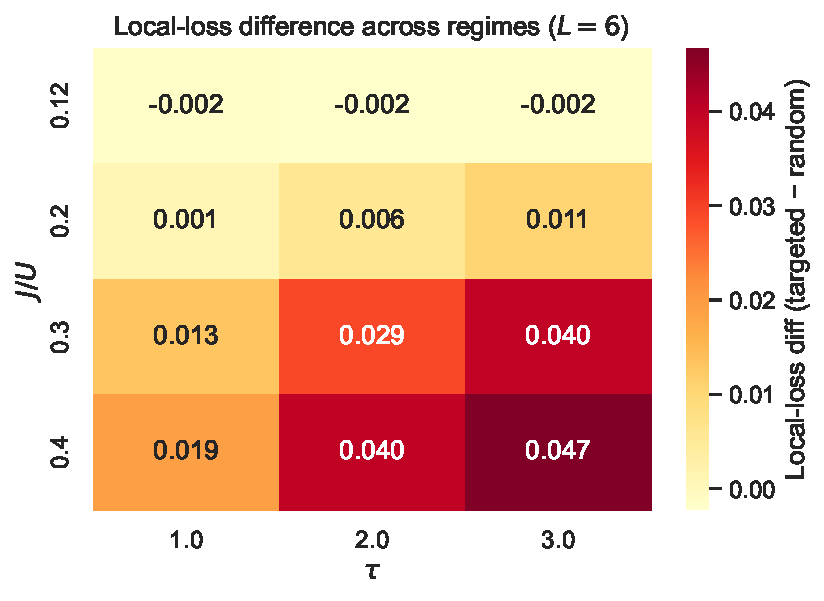
\includegraphics[width=0.85\linewidth]{fig1_main_heatmap.pdf}
\caption{Local-loss difference across $J/U$ and $\tau$ at $L=6$.
The handle effect is positive in the intermediate and stronger coupling
regime and absent or reversed at the lowest tested coupling.}
\label{fig:main_heatmap}
\end{figure}

\subsection{Robustness across chain length}

Table~\ref{tab:robust} shows pooled results at $J/U\in\{0.30,0.40\}$
for $L\in\{6,7\}$.
The positive pocket at $J/U\in\{0.30,0.40\}$ passes at all four tested
chain lengths $L\in\{6,7,8,9\}$ with 95\% confidence intervals excluding
zero at every horizon $\tau\in\{1,2,3\}$, confirming that the positive
pocket is not a small-size artefact.

The intermediate coupling $J/U=0.20$ is strongly size-sensitive: it passes
at $L=6$ across all horizons, requires $\tau=3$ at $L=7$, passes only at
$\tau\in\{2,3\}$ at $L=8$, and fails at all tested horizons at $L=9$.
This size-dependent behaviour places $J/U=0.20$ squarely in the crossover
band rather than the robust positive pocket (see Sec.~\ref{sec:onset}).

\begin{table}[tbp]
\centering
\caption{Pooled local-loss difference for $L\in\{6,7\}$ at
$J/U=0.30$ and $0.40$ (two representative sizes from the full ladder).
Format: mean $[\text{95\% CI}]$, pooling trial-level differences across
$\tau\in\{1,2,3\}$.
All four tested sizes $L\in\{6,7,8,9\}$ pass at both couplings (see text).}
\label{tab:robust}
\input{outputs/tables/table_robust.tex}
\end{table}

\begin{figure}[tbp]
\centering
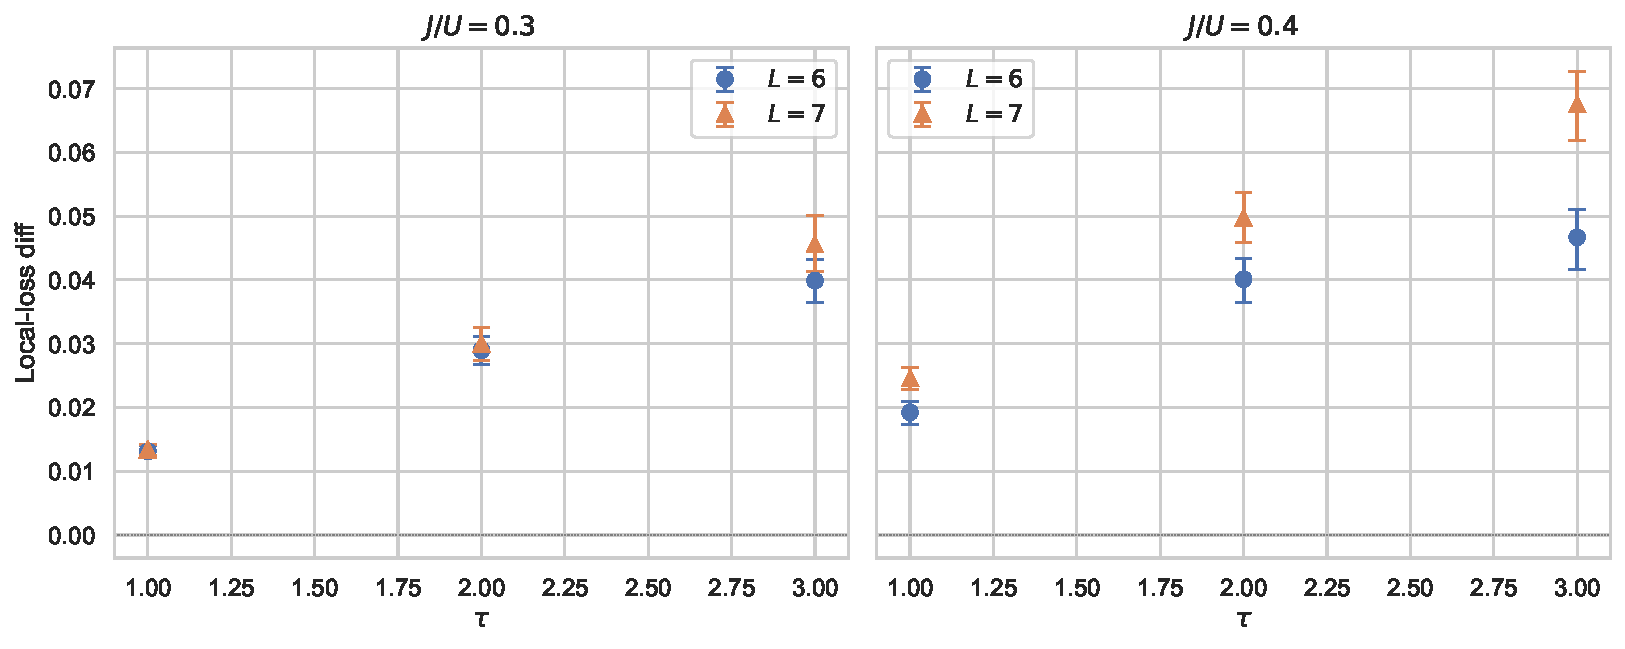
\includegraphics[width=0.85\linewidth]{fig2_robustness.pdf}
\caption{Local-loss difference at $J/U=0.30$ and $0.40$ for
$L=6$ and $L=7$ (two representative sizes). Error bars are 95\% bootstrap CIs.
The same positive result holds at $L=8$ and $L=9$; the positive pocket
is robust across the full size ladder $L\in\{6,7,8,9\}$.}
\label{fig:robustness}
\end{figure}

\subsection{Regime map}
\label{sec:regime}

The results define three regimes within the tested parameter range:

\textbf{Negative regime} ($J/U=0.12$):
The targeted intervention produces less local loss than random targeting at
all four chain lengths and all horizons.
In this deep Mott-like regime the occupation-variance handle does not
identify causally effective sites; the 95\% CIs are strictly negative at
every $(L,\tau)$ combination tested.

\textbf{Crossover band} ($J/U\approx0.18$--$0.24$, depending on $L$ and $\tau$):
The handle begins to function but its effectiveness is size- and
horizon-dependent.
The first-pass onset shifts upward with $L$ (for fixed $\tau$) and
downward with $\tau$ (for fixed $L$), both trends monotone across the
ladder (see Sec.~\ref{sec:onset}).

\textbf{Positive pocket} ($J/U\gtrsim0.30$):
The handle is consistently positive across all four chain lengths and all
horizons $\tau\in\{1,2,3\}$.
This is the regime where the occupation-variance selector reliably
identifies sites whose perturbation produces excess local loss, with CIs
strictly above zero at every tested $(L,\tau)$ combination.

The existence of a negative boundary regime and a structured crossover band
is itself informative: the handle is not a generic property of the dephasing
operator but is sharply regime-dependent.

\subsection{Crossover-band onset}
\label{sec:onset}

The boundary sweep resolves the smallest $J/U$ at which the 95\% CI first
strictly excludes zero (first PASS) for $L\in\{8,9\}$.
Table~\ref{tab:onset} reports these onset couplings for horizons
$\tau\in\{2,3\}$.

\begin{table}[tbp]
\centering
\caption{First-PASS onset coupling: smallest $J/U$ at which the 95\% CI
strictly excludes zero, by chain length $L$ and horizon $\tau$.
Entries $\leq\!0.20$ are bounded by the initial sweep (exact onset lies
in the interval $(0.12,\,0.20]$); entry $>\!0.20$ indicates a failure at
$J/U=0.20$ with onset in $(0.20,\,0.30)$ (not resolved by the boundary
sweep, which focused on $L\geq8$).}
\label{tab:onset}
\begin{ruledtabular}
\begin{tabular}{ccc}
$L$ & $\tau=2$ & $\tau=3$ \\
\colrule
$6$ & $\leq0.20$ & $\leq0.20$ \\
$7$ & $>0.20$    & $\leq0.20$ \\
$8$ & $0.20$     & $0.18$     \\
$9$ & $0.24$     & $0.22$     \\
\end{tabular}
\end{ruledtabular}
\end{table}

The onset coupling is monotonically increasing with $L$ for fixed $\tau$,
and monotonically decreasing with $\tau$ for fixed $L$, across the full
tested range.
The convergence of these two trends in the range
$J/U\approx0.18$--$0.24$ defines the empirical crossover band reported
in the abstract.
In particular, any coupling in $J/U\gtrsim0.30$ lies above the onset for
all tested $(L,\tau)$ combinations, consistently defining the positive
pocket boundary.

\subsection{Spatial response pattern}

Fig.~\ref{fig:mechanism} shows the site-resolved occupation change under
targeted versus random intervention at $J/U=0.30$, $L=6$, $\tau=2$.
The bars show the mean site-resolved occupation change under the
deterministic targeted intervention and averaged across the 100
matched-budget random interventions.

The observed pattern is consistent with a nonlocal, redistributive
response.
Under targeted intervention, the selected sites (shaded) tend to show
\emph{less} negative occupation change than under random intervention:
selected-site loss is reduced relative to random targeting.
At the same time, non-selected sites show increased occupation loss under
targeted intervention.
The net effect is that the intervention changes the spatial pattern of
occupation change across the chain rather than simply amplifying loss at
the targeted sites themselves.

This is the opposite of what a purely local-instability mechanism would
predict, in which extra dephasing at a high-$\Fi$ site would increase loss
specifically at that site.
The data are more consistent with a picture in which perturbing high-$\Fi$
sites alters the subsequent spatial distribution of occupation change
across the chain.

\begin{figure}[tbp]
\centering
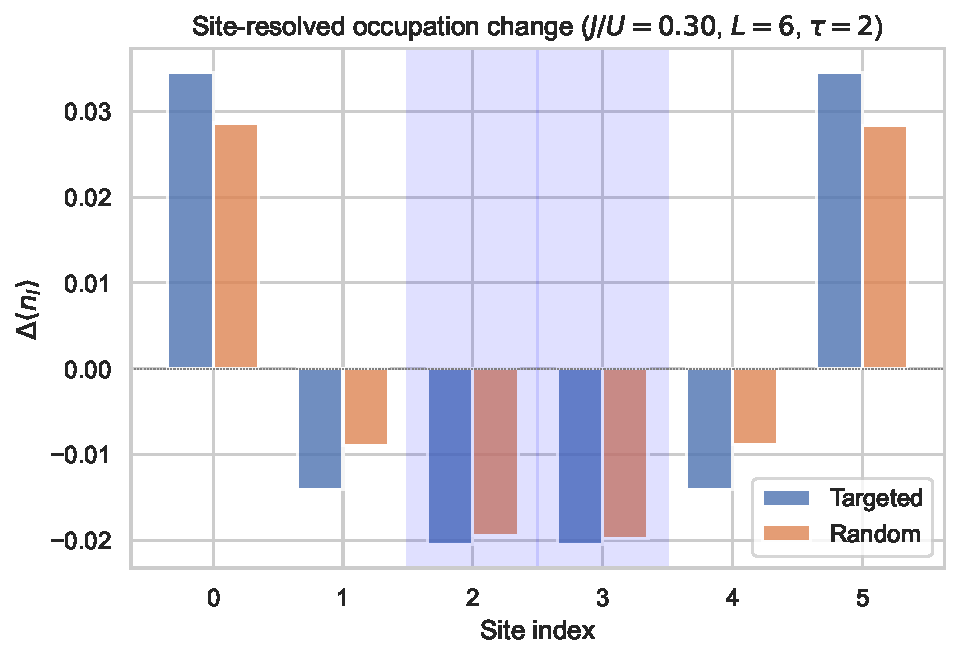
\includegraphics[width=0.85\linewidth]{fig3_mechanism.pdf}
\caption{Mean site-resolved occupation change under the targeted
intervention and across matched-budget random interventions
($J/U=0.30$, $L=6$, $\tau=2$).
Negative values correspond to occupation loss.
Shaded bands mark selected sites.
The spatial response is consistent with nonlocal redistribution.}
\label{fig:mechanism}
\end{figure}

\section{Discussion}
\label{sec:disc}

\paragraph{Summary.}
In an open Bose--Hubbard chain, sites of high local occupation variance
serve as causal handles in the intermediate and stronger coupling regime:
targeting them with additional dephasing produces more local future
occupation loss than matched-budget random targeting at
$J/U\in\{0.30,0.40\}$, robustly across the full tested size ladder
$L\in\{6,7,8,9\}$ and all tested horizons $\tau\in\{1,2,3\}$.
The effect is absent or reversed in the negative regime ($J/U=0.12$) and
size- and horizon-dependent in the crossover band
$J/U\approx0.18$--$0.24$, with the first-pass onset shifting upward with
$L$ and downward with $\tau$, both trends monotone across the ladder.

\paragraph{Mechanism.}
The site-resolved response is more consistent with nonlocal redistribution
than with local instability.
Perturbing high-$\Fi$ sites is associated with a redistribution of
subsequent occupation change across the chain.
A complete mechanistic account is beyond the scope of the present analysis.

\paragraph{What is not claimed.}
We do not claim that high-$\Fi$ targeting is optimal among all possible
intervention strategies; that the effect extends to all coupling regimes
(it does not hold at $J/U=0.12$ and is transitional in the crossover band
$J/U\approx0.18$--$0.24$); that the mechanism generalises to other quantum
systems or to chains beyond the tested range; or that the
occupation-variance handle corresponds to any equilibrium observable.

\paragraph{Scope and limitations.}
The causal-handle effect is regime- and size-dependent in the present
design, with the clearest fully robust support in the
$J/U=0.30$--$0.40$ regime.
The Hilbert-space dimension of the fixed-$N$ sector grows combinatorially
with $L$ and $n_{\max}$, limiting exact Lindblad evolution to small chains.
The tested range ($L\leq9$, $n_{\max}=3$) establishes the effect in the
positive pocket and sharpens the crossover band to
$J/U\approx0.18$--$0.24$ (depending on system size and horizon),
but does not access the thermodynamic limit.
Whether the positive pocket persists, broadens, or shifts at larger system
sizes is an open question requiring approximate methods such as
matrix-product-operator Lindblad evolution~\cite{daley2014}.

\paragraph{Experimental relevance.}
The 1D open Bose--Hubbard model under dephasing is experimentally
motivated.
Cold-atom optical-lattice platforms already realise 1D Bose--Hubbard-like
systems with tunable $J/U$~\cite{jaksch1998,greiner2002}, and recent
advances in quantum-gas microscopy provide site-resolved preparation and
readout relevant to the targeted-intervention protocol studied
here~\cite{gross2021}.
In particular, groups working with 1D optical lattices have demonstrated
single-site addressing and out-of-equilibrium dynamics in regimes that
overlap with the coupling range explored here.
The Lindblad dephasing modelled by $\gamma\hat{n}_i$ is a standard
approximation for photon-scattering-induced decoherence in optical
lattices~\cite{pichler2010,daley2014}.
The present results therefore constitute a theory-side proposal with
experimental plausibility: the positive-pocket and crossover-band
structures identified here are, in principle, accessible to existing
site-resolved cold-atom platforms, though the exact causal-handle
protocol has not yet been implemented experimentally.

\begin{acknowledgments}
The author thanks the open-source scientific Python community for the
libraries underlying this work: NumPy, SciPy~\cite{scipy2020}, pandas,
matplotlib, and tqdm.
\end{acknowledgments}

\section*{Data and Code Availability}

All simulation code and raw data are available at
\href{https://github.com/kunalb541/BH}{github.com/kunalb541/BH}.

\bibliography{refs}

\end{document}
